% \chapter{Trabajo}

% Preface
% \note{Soy un estudiante italiano en Erasmus. Hablo español bastante bien, pero me resulta más natural escribir en inglés; sin embargo, decidí escribir en español para practicar, con la ayuda de algunos traductores cuando era necesario. Si hay algo mal escrito o poco claro, estoy a disposición para cualquier aclaración.}

\chapter{Trabajo académico - Planificación Inteligente}

\lstset{language=python}


% \note{Sé que un mi compañero prenguntó si podía escribir en inglés, y que está bien; hablo bastante bien español y habeis empezado pero Me resulta más confortable y natural escribir en inglés, y creo que sea mejor que confiar en ChatGPT (y similares) para la corrección de la traducción \smiley.}

\note{Sé que un mi compañero prenguntó si podía escribir en inglés, y que está bien; Soy un estudiante italiano en Erasmus. Hablo español bastante bien, pero me resulta más natural escribir en inglés; sin embargo, decidí escribir en español para practicar, con la ayuda de algunos traductores cuando era necesario. Si hay algo mal escrito o poco claro, estoy a disposición para cualquier aclaración.}

\section{Introducción}

He eligido el \textbf{dominio de emergencias} para mi trabajo. Resumiendo lo que está escrito en la tarea, en este dominio los puntos de interés son los siguientes:
\begin{itemize}
   \item Localización de las víctimas, ambulancias y hospitales.
   \item Asignación de ambulancias a las víctimas, teniendo en cuenta la gravedad de la emergencia.
   \item Minimización del tiempo de respuesta, como objetivo.
\end{itemize}

La version más basica del escenario incluye una sola víctima, en vez la version ampliada mas victímas.

\section{Implementación}

\subsection{Organización del código}
El código se divide en tres ficheros:
\begin{itemize}
   \item \texttt{emerg.py}: contiene la implementación de las funciones de los operadores y métodos.
   \item \texttt{scenario.py}: contiene la definición del estado inicial.
   \item \texttt{utils.py}: contiene funciones auxiliares, para trazar el grafico de la ciudad de Valencia y imprimir algunos mensajes.
\end{itemize}

\texttt{//TODO dockerize}

Para ejecutar el código se puede usar el comando \texttt{python3 emerg.py}, o si lo prefiere puede utilizar Docker, para evitar la instalación de las dependencias necesarias.

\subsection{Representación del estado}
El estado se representa con alguno diccionarios, uno para cada entidad:
\begin{lstlisting}
   state1.ambulances = [ {'label': 'A1', 'cap': 10, 'loc': 'El Carmen'},...
   state1.victims = [ {'name': 'Carlos', 'sev': 5, 'loc': 'El Carmen'},...
   state1.hospitals = [ {'name': 'H1', 'loc': 'Hospital La Fe'},...
\end{lstlisting}
En cada entrada del diccionario se encuentran propiedades de la entidad como la posición, el nombre y la gravedad.

Las localidades son barrios de la ciudad de Valencia, y cada barrio es caracterizado por coordenadas \lstinline|(X,Y)|.
Se asume que es posible viajar entre cualquier par de localizaciones y el tiempo de viaje es proporcional a la distancia euclídea entre ambas.
\begin{figure}[htbp]
   \centering
   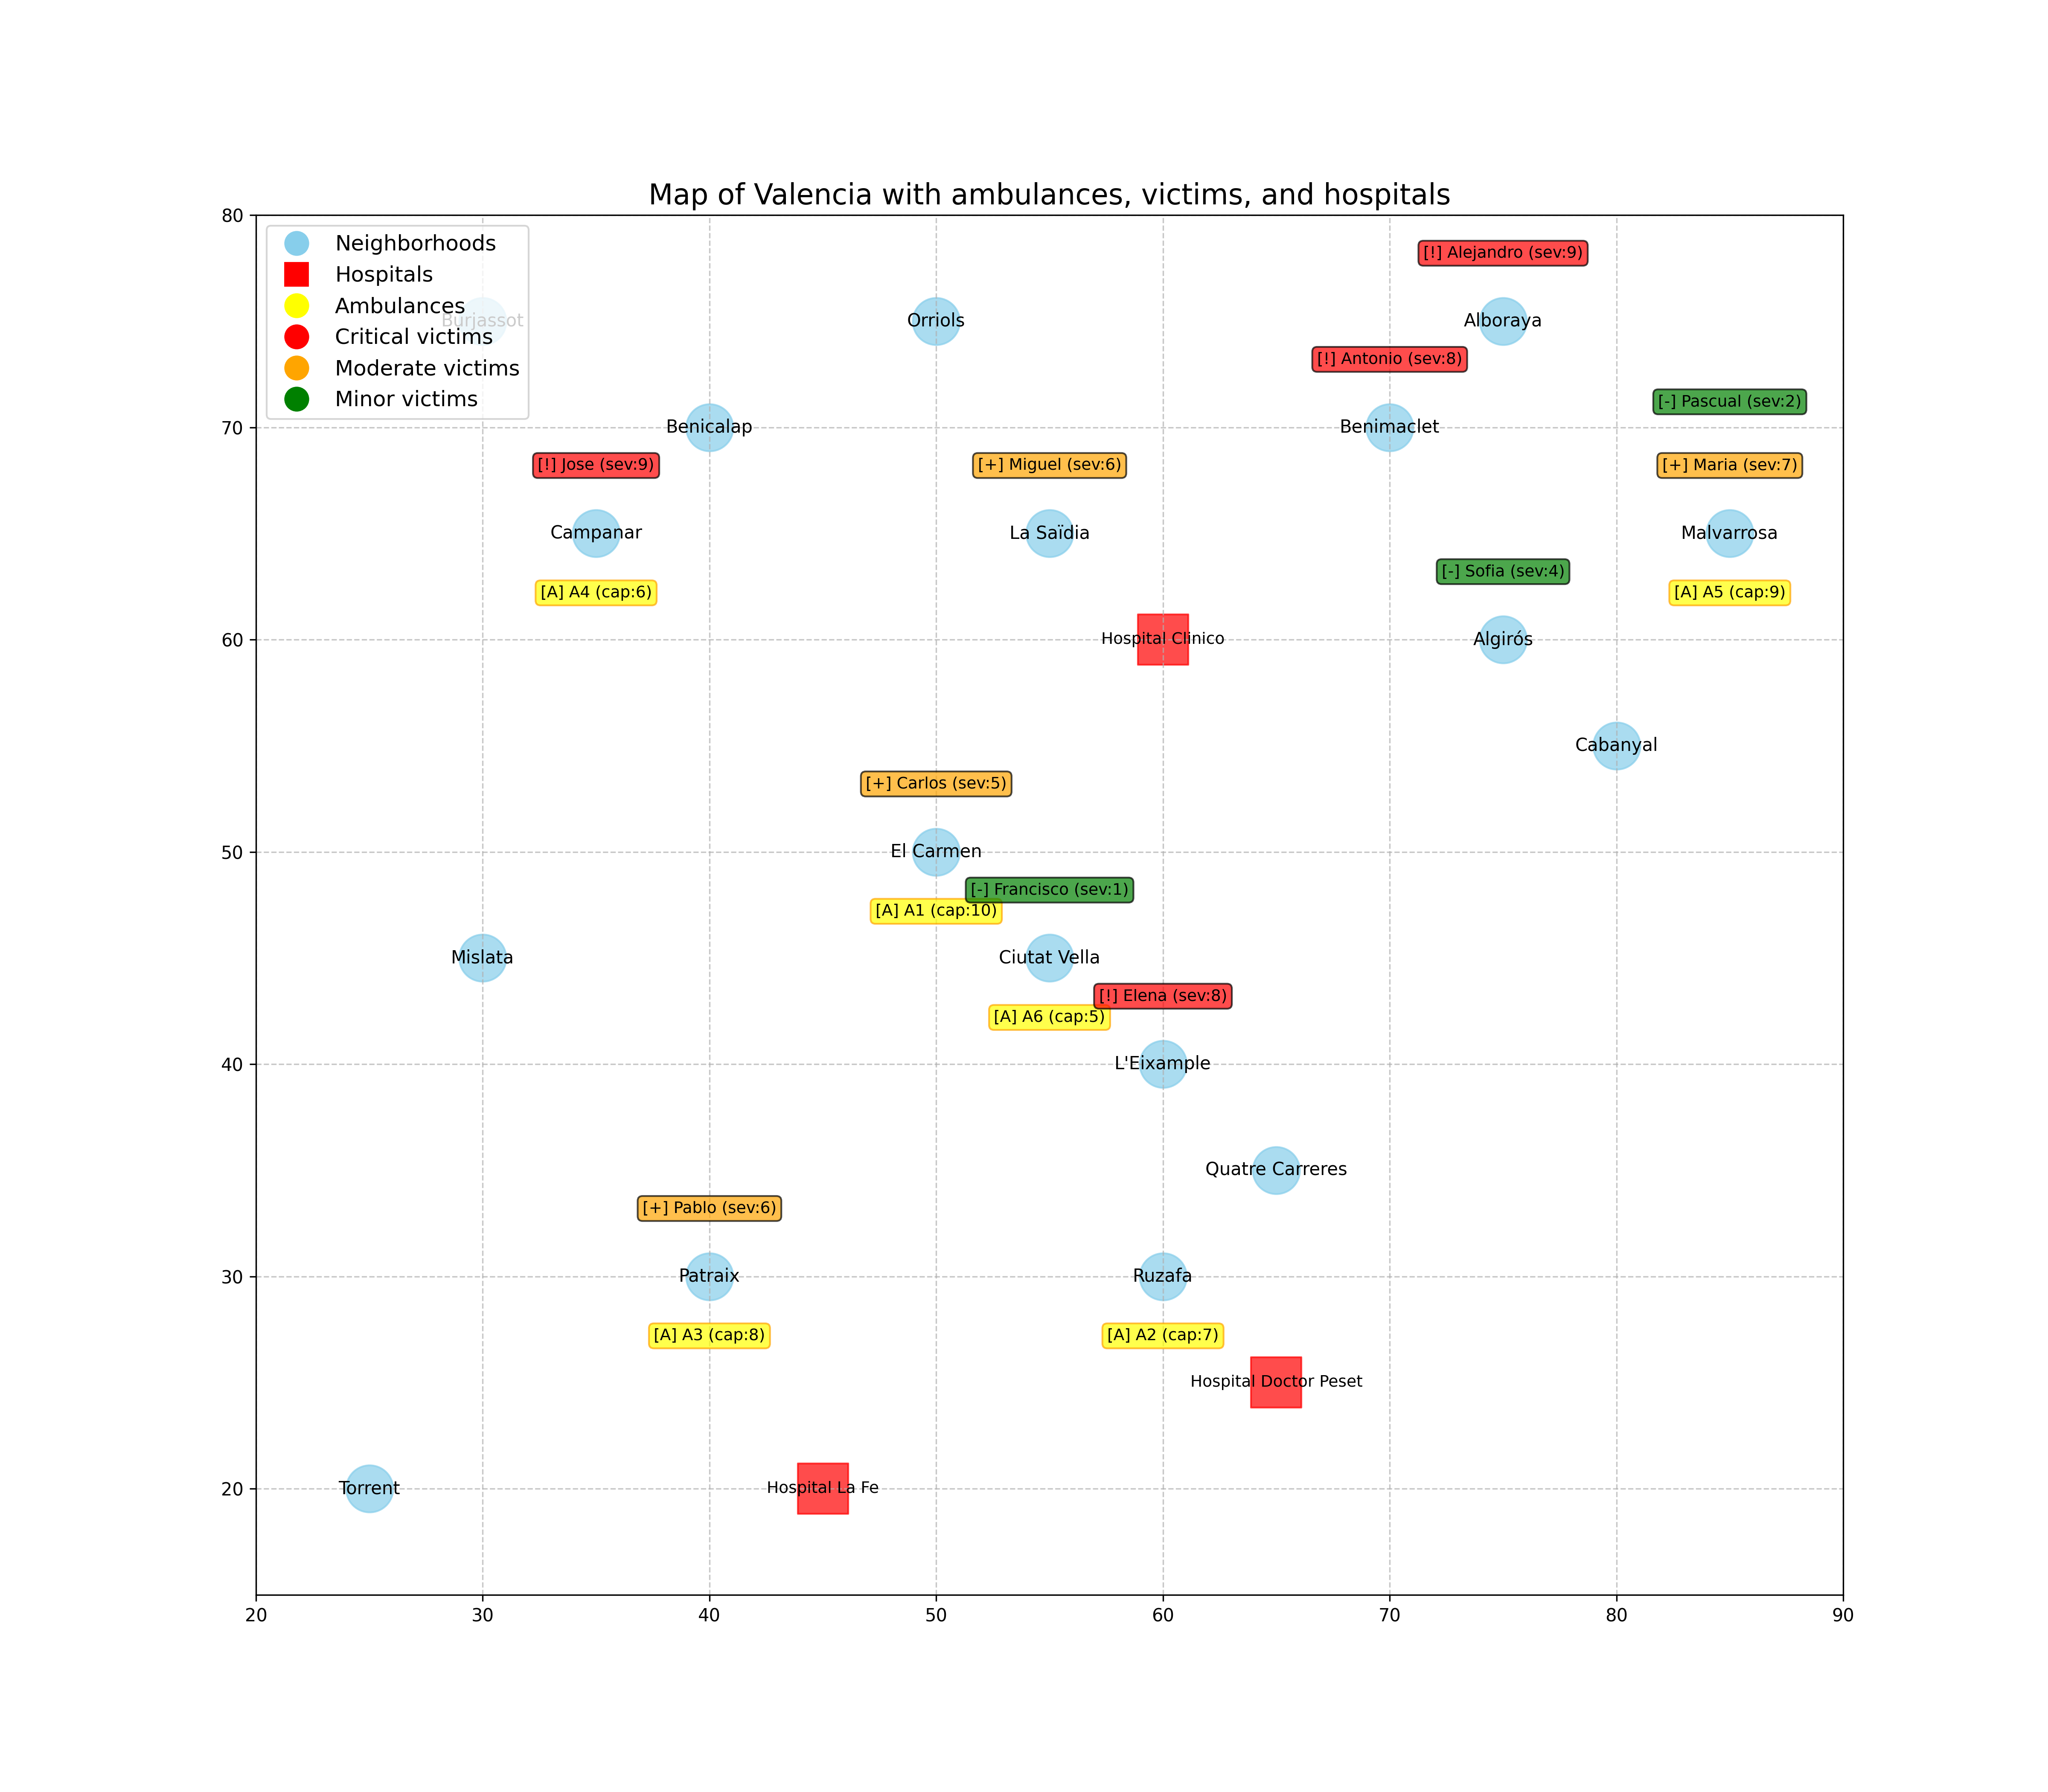
\includegraphics{images/valencia_map.png}
   \caption{Barrios de Valencia}
   \label{fig:valencia_map}
\end{figure}

\subsection{Operadores}

Los operadores de pyhop representan las acciones que se pueden realizar en el dominio, y no so se pueden descomponerse. Se devuelve al nueve estado tras aplicarse el operador o \lstinline|False| si el operador falla (i.e. no se aplicable).
Entonces los operadores en nuestro dominio son lo siguientes, que son bastante self-explanatory:
\begin{itemize}
   \item \lstinline|op_drive(state, amb, dest)| - Mover la ambulancia a una localización. Puede parecer complicado pero es solo porque hay algunas instrucciones para trazar el camino en el mapa. No es necesario para la planificación, pero es útil para la visualización. 
   \item \lstinline|op_load(state, amb, victim)| - Cargar una víctima en una ambulancia. Aquí tenemos que verificar que la ambulancia tiene suficiente capacidad para la severidad de la víctima.
   \note{Nel código esto control se hace también en el método \lstinline|method_deliver_victim|.}
   \item \lstinline|op_unload(state, amb, victim, hospital)| - Descargar una víctima en un hospital.
   \item \lstinline|op_treat(state, amb, victim)| - Tratar a una víctima en una ambulancia si su gravedad supera el umbral de la primera asistencia.
   \item \lstinline|op_remove_victim(state, victim_name)| - Solo remueve la víctima de la lista de víctimas.
\end{itemize}

\subsection{Métodos}

Los métodos implementan la logica de la planificación, y determinan la secuencia de operadores que se deben aplicar para alcanzar un objetivo.

El método fundamental es \lstinline|method_deliver_victim(state, victim_dict, hospital)|, que se utiliza por mover la ambulancia más cercana a la víctima, cargar la víctima, mover la ambulancia al hospital y descargar la víctima.
Este método es lo más sencillo, y es invocado por los otros métodos para resolver el problema de las víctimas múltiples.


La manera más intuitiva y sencilla de implementar la gestión de multiple victímas es de llamar recursivamente el método de búsqueda para cada victima, escribiendo algo así:
\begin{lstlisting}[caption={Esto no se encuentra en el código entregado}, captionpos=b]
   def method_deliver_all(state):
   if not state.victims:
       return []  # Base case: no more victims to deliver.
   
       # Take the first victim in the list.
       victim = state.victims[0]
       return [('deliver_victim', victim, 'H1'),
           ('op_remove_victim', victim['name']),
           ('deliver_all',)]
\end{lstlisting}

Sin embargo, el orden en que se entregan las víctimas afecta a la travel distance, porque el estado de las ambulancias cambia después de cada entrega, entonces, la solucción óptima no es la misma que la solucción de los subproblemas.\\
Parece claro que el orden en que se entregan las víctimas afecta a la travel distance;
las instrucciones del trabajo no piden específicamente tratar este tema, pero me intrigó y pensé que merecía la pena analizarlo.

He implementado cuatro métodos para entregar todas las víctimas, que vamos a describir más detalladamente abajo en la Sec. \ref{sec:ordenar_victimas}.
\begin{itemize}
   \item \lstinline|method_deliver_all_distance_priority(state)| - Entregar todas las víctimas en orden de distancia a la ambulancia más cercana.
   \item \lstinline|method_deliver_all_severity_priority(state)| - Entregar todas las víctimas en orden de severidad.
   \item \lstinline|method_deliver_in_order(state)| - Entregar las víctimas en el orden en que se encuentran en la lista.
   \item \lstinline|try_all_permutations(state, max_victims=5)| - Probar todas las permutaciones de las víctimas y devolver la que minimiza la distancia total recorrida y la que minimiza el \textit{makespan}.\\
   Parece complicado da leer, pero en realidad es bastante simple, solo tiene que manejar distintas variables de tracking para controlar las permutaciones y las distancias.
   \note{Hay un umbral \lstinline|max_victims| para limitar el número de permutaciones que se prueban, porque el número de permutaciones crece muy rápidamente con el número de víctimas. Sobre el umbral se generan solo \lstinline|max_victims!| permutaciones, y se eligen casualmente.}
\end{itemize}

\section{Observaciones}

\subsection{Ordenar víctimas}
\label{sec:ordenar_victimas}

Antes de decidir como ordinar las victímas es necesario definir un criterio de optimización. He considerado tres posibles funciones objetivo:
\begin{enumerate}
   \item \textbf{Severidad} de emergencia - Prioritizar las víctimas más graves: esto es ---más o menos--- lo que se prefiere hacer en un escenario real, sin embargo, no conduce a minimizar la distancia de viaje\footnote{Puede ocurrir, pero por casualidad.}.
   Esta función objetivo es la más fácil de implementar, porque se puede ordenar la lista de víctimas por severidad y luego entregarlas en ese orden, no hay muchas decisiones que tomar, solo que la ambulancia más cercana a la víctima se mueve a su localización.
   \begin{lstlisting}
   def method_deliver_all_severity_priority(state):
      if not state.victims:
          return []  # Base case: no victims left
      # Sort victims by severity (most severe first)
      victims_by_severity = sorted(state.victims, key=lambda v: v['sev'], reverse=True)
      victim = victims_by_severity[0] # The most severe victim
      best_hosp = # The closest hospital
      return [('deliver_victim', victim, best_hosp['name']),
              ('method_deliver_all_severity_priority',)]
   \end{lstlisting}
   \item \textbf{Travel distance} - Minimizar la distancia total recorrida por las ambulancias. Para hacer esto he implementado un algoritmo \textit{greedy}, que elige primero la víctima que tiene la más cercana ambulancia. 
   \begin{lstlisting}
   def method_deliver_all_distance_priority(state):
      # ...
      for victim in state.victims:
         for amb in state.ambulances:
             if amb['cap'] >= victim['sev']:  # Ambulance can handle this victim
                 dist = euclidean_distance(amb['loc']),victim['loc'] ))
                 if dist < min_distance:
                     min_distance = dist
                     best_victim = victim
      # ...
   \end{lstlisting}

   No estaba seguro de si esto garantizaba la solución óptima, así que intenté enumerar todas las permutaciones de víctimas y calcular la distancia total para cada permutación, y parece ---salvo errores en la implementación ---que la solución greedy ya proporciona la distancia óptima.\\
   Para hacer esto hay el método \lstinline|try_all_permutations(state, max_victims=5)|, que prueba todas las permutaciones, y se puede observar como la mejor solucción que encuentra es la misma que la solucción greedy.

   \note{No he probado todas las permutaciones de ambulancias para cada victima en cada permutación, he utilizado como criterio de elección de la ambulancia lo mismo que en los otros métodos, la ambulancia más cercana a la victima.}
   \item \textbf{Makespan} - Asumiendo como dice el texto que el tiempo de viaje es proporcional a la distancia euclídea entre dos localizaciones, se puede considerar que dos ambulancias distintas pueden viajar simultáneamente, entonces, el tiempo total de respuesta es el tiempo que tarda la última ambulancia en llegar al hospital.\\
   Un buen algoritmo para minimizar el makespan puede ser de utilizar el mayor número posible de ambulancias, pero no he implementado este método. En vez, se observa que, como es lógico, en relación con el makespan, las permutaciones casuales pueden ofrecer a menudo mejores resultados que el algoritmo greedy utilizado para minimizar \textit{travel distance}.
\end{enumerate}

\subsection{Estados iniciales}

En \texttt{scenario.py} se definen cuatro estados iniciales
\begin{enumerate}
   \item Una sola víctima
   \item 5 víctimas, donde todas las permutaciones de las víctimas son evaluadas.
   \item 10 víctimas, que no permite de evaluar todas la permutaciones, solo algunas eligidas casualmente, y en efecto observamos cómo distintas ejecuciones dan resultados diferentes.
   \item 5 víctimas que tiene que fallar porque no hay ninguna ambulancia capaz de transportar a la víctima más grave.
\end{enumerate}

\section{Conclusiones}

El problema de la planificación de emergencias es un problema interesante y complejo, y se puede complicar más si se van a consider multiplés funciones objetivo.
En uno escenario real, la severidad de la emergencia es importante, pero no es el único factor a considerar, es necesario también minimizar el tiempo de respuesta para todas la víctimas.\\
En general, he leido online que el \textit{Emergency Vehicle Dispatching Problem} es una variante del \href{https://en.wikipedia.org/wiki/Vehicle_routing_problem}{\textit{Vehicle Routing Problem}} (VRP), que es un problema NP-hard, que pero parece diferir dal nuestro problema en algunos aspectos, sobre todo que en el VRP hay un grafo con arcos que tienen un costo asociado y que determinen entre cuales nodos se puede viajar, mientras en nuestro problema se puede viajar entre cualquier par de nodos. Podemos imaginar que el nuestro es un caso particular en que el grafo es completo.

Y además, en la realidad, no siempre todos los hospitales están disponibles, el trafico afecta a la travel distance, y otros factores tecnicos (carburante, turnos de trabajo, mantenimiento de vehículos, \dots) y éticos/humanos pueden influir en la solucción elegida.

